\section{Introduction}
Modern robotic systems, including manipulators, mobile robots, and soft robots,
exhibit strongly nonlinear dynamics due to mechanical coupling, actuator
effects, and uncertain interactions with the environment~\cite{Brunton2022,DellaSantina2023}.
Accurate dynamic models are essential for high-performance control, yet
first-principles modeling becomes difficult when a robot contains flexible
structures, uncertain parameters, or unmodeled interactions~\cite{Mamakoukas2021TRO}.
Data-driven models learned from operational data therefore provide an attractive
alternative for robotic prediction and control~\cite{Brunke2022,Tang2025survey,LiSu2026TCST,LiEtAl2026TCYB}.

Koopman operator theory offers a control-oriented way to
represent nonlinear dynamics by linear evolution in a lifted observable
space~\cite{Koopman1931,Korda2018conv}. Since the Koopman operator is
infinite-dimensional, practical methods rely on finite-dimensional
approximations. EDMD constructs such an
approximation by lifting the state through a user-specified dictionary of basis
functions~\cite{Williams2015EDMD,Korda2018conv}. The resulting lifted linear
models enable the use of linear-system tools, including Koopman-based model
predictive control and Koopman-based linear quadratic regulation, for nonlinear
robotic systems~\cite{Proctor2016DMDc,Korda2018MPC,Brunton2016Koopman}.

A key bottleneck of EDMD is the choice of basis functions.
In principle, the dictionary should span a subspace that is approximately
invariant under the Koopman operator. In practice, constructing such a
dictionary requires substantial prior knowledge of the underlying dynamics
\cite{Mauroy2019}. This leads to a tradeoff: a small dictionary may miss
important nonlinear features, whereas an overcomplete dictionary increases
computational cost, introduces redundancy and ill-conditioning, and may cause
overfitting~\cite{Mamakoukas2021TRO,ShiKarydis2022RAL}.

Two common strategies are learned dictionaries and sparse selection. Deep
learning methods can learn nonlinear coordinates from
data~\cite{Lusch2018,ShiMeng2022RAL,Ren2023TMech}, but the resulting features
are often difficult to interpret and analyze in robotic control. For example,
EDMDDL learns a
nonlinear dictionary for the Koopman operator~\cite{Li2017}. Sparse regression
methods select compact representations from large libraries~\cite{Zhang2022Automatica},
but they may involve nonsmooth optimization and sensitivity to noise and
hyperparameters~\cite{WangEtAl2023RAL}. For robotic systems, it is therefore
desirable to retain the interpretability of physics-informed candidate functions
while avoiding the computational burden of using the full overcomplete
dictionary.

We therefore retain an overcomplete, physics-informed candidate library and
learn a lower-dimensional recombination of its functions. An optimizable
selection matrix parameterizes this recombination, and the resulting FS-EDMD
model is trained directly for lifted
one-step prediction. Unlike PCA, which preserves dominant data variance, our
objective targets the prediction error that matters for control. The Koopman and
selection matrices are then updated jointly by block coordinate descent with
convergence guarantees. Using the learned lifted model, we design a
feedforward-feedback Koopman-LQR controller for trajectory tracking. The
finite-dimensional approximation error is treated as a bounded disturbance,
allowing the closed-loop tracking error to be analyzed through Lyapunov
arguments.

The main contributions are summarized as follows.
{\renewcommand{\labelenumi}{(\arabic{enumi})}
\begin{enumerate}
\item We propose a feature-selection-based framework for Koopman
representation learning in robotic systems. A physics-informed overcomplete
candidate library is constructed, and a learnable feature selection matrix is
embedded into the lifted state. This yields compact and informative feature
combinations while preserving the interpretability of the candidate library.

\item The Koopman modeling task is formulated as a joint optimization problem
over the Koopman matrices and the feature selection matrix. The resulting
problem is solved by a block coordinate descent algorithm, where the matrix
update subproblems are explicitly characterized and convergence to a
stationary point is established under standard assumptions.

\item A robust feedforward-feedback Koopman-LQR controller is developed for
robotic trajectory tracking. By modeling finite-dimensional Koopman
approximation errors and external uncertainties as bounded lumped
disturbances, Lyapunov analysis proves that the closed-loop tracking error is
ultimately uniformly bounded and relates disturbance level to the
steady-state tracking bound.

\item The proposed modeling and control framework is validated on two robotic
platforms with distinct dynamics: a three-degree-of-freedom rigid robot arm and
a cable-driven soft platform. The experiments evaluate multi-step model
prediction, trajectory tracking on several reference patterns, and disturbance
recovery.
\end{enumerate}}

The rest of this paper is organized as follows. Section~\ref{sec:background}
introduces the preliminaries of Koopman operator theory and formulates the
problem considered in this paper. Section~\ref{sec:koopman} presents the
feature-selection-based Koopman representation learning framework and the
corresponding block coordinate descent algorithm. Section~\ref{sec:lqr}
develops the Koopman-based feedforward-feedback LQR controller and analyzes
the closed-loop robust tracking performance. Section~\ref{sec:experiments}
reports prediction and control experiments on both robotic platforms.
Finally, Section~\ref{sec:conclusion} concludes this paper.

\textit{Notation:} Unless otherwise stated,
$\|\cdot\|$ denotes the Euclidean norm for vectors and the induced $2$-norm
for matrices, $\|\cdot\|_1$ denotes the $\ell_1$ norm, and $\|\cdot\|_F$
denotes the Frobenius norm for matrices; $\mathbb{R}^n$ denotes the
$n$-dimensional Euclidean space; the superscripts $(\cdot)^\top$ and
$(\cdot)^\dagger$ denote the transpose and the Moore--Penrose pseudoinverse,
respectively; $\I_n$ denotes the $n \times n$ identity matrix;
$\mathbf{0}_{m \times n}$ denotes the $m \times n$ zero matrix;
$\tr(\cdot)$, $\rank(\cdot)$, and $\diag(\cdot)$ denote the trace, rank, and
diagonal matrix operator, respectively; $\mathcal{K}$ denotes the Koopman
operator; $\mathcal{H}$ denotes a Hilbert space; $\Phib(\x)$ denotes the
feature library; for a matrix $\mathbf{A}$, $\mathbf{A} \succeq 0$ and
$\mathbf{A} \succ 0$ mean that $\mathbf{A}$ is positive semidefinite and
positive definite, respectively.


% =========================================================
\section{Preliminaries and problem formulation}
\label{sec:background}
% =========================================================

\subsection{Koopman Operator Theory}
\label{subsec:koopman_theory}

Consider the discrete-time nonlinear system
\begin{equation}
\x_{k+1} = f(\x_k, \uvec_k),
\end{equation}
where $\x_k \in \R^n$ is the system state and $\uvec_k \in \R^m$ is the control input at time step $k$. The mapping $f: \R^n \times \R^m \to \R^n$ describes the state transition. It is assumed that $f$ is Lipschitz continuous on its domain.

Let \(\mathcal{H}\) be a Hilbert space of real-valued observation functions defined on the state space. For any observation function \(g \in \mathcal{H}\), when the control input is \(\uvec_k\), the discrete-time Koopman operator \(\mathcal{K}: \mathcal{H} \to \mathcal{H}\) is defined by the evolution of \(g\) along the system trajectories as
\begin{equation}
(\mathcal{K}g)(\x_k,\uvec_k) \triangleq g(f(\x_k,\uvec_k)) = g(\x_{k+1}).
\end{equation}

The core of Koopman operator theory is to lift the nonlinear dynamics
from the finite-dimensional state space to an infinite-dimensional
function space $\mathcal{H}$, thereby achieving linear evolution that
obeys the superposition principle:
\begin{equation}
\mathcal{K}(\alpha g_1 + \beta g_2) = \alpha \mathcal{K}g_1 + \beta \mathcal{K}g_2,
\end{equation}
where $g_1, g_2 \in \mathcal{H}$ are arbitrary observation functions and $\alpha, \beta \in \mathbb{R}$ are arbitrary
scalars. This linearity enables the application of linear-system tools to analyze
nonlinear dynamics after lifting.

\subsection{Problem Formulation}
\label{subsec:motivation}
As $\mathcal{H}$ is typically infinite-dimensional, EDMD approximates the Koopman operator in a finite-dimensional space spanned by a candidate function library $\{g_i\}_{i=1}^M$. The approximation quality depends critically on this library. A small library may miss essential nonlinear features, whereas an overcomplete library increases computational cost and may introduce redundancy and overfitting.

This accuracy--complexity tradeoff constitutes a central challenge in basis function selection for EDMD and related data-driven Koopman methods. To address this challenge and enable practical robotic control, this paper aims to: (1) learn a compact Koopman lifted representation from a physics-informed overcomplete candidate function library by using a feature selection matrix; and (2) design a robust feedforward-feedback LQR controller based on the learned lifted model to achieve reliable trajectory tracking under bounded lumped disturbances.


% =========================================================
\section{Koopman Representation Learning Based on Feature Selection Mechanism}
\label{sec:koopman}
% =========================================================

This section develops the feature-selection-based Koopman learning framework, including the joint optimization algorithm and the lumped-disturbance model used for robust control.

% ---------------------------------------------------------
\subsection{Learnable Feature Selection and Joint Optimization}
\label{subsec:algorithm}
% ---------------------------------------------------------
We first construct an overcomplete candidate observation function library $\Phib(\x):\R^n\to\R^P$, where $P\gg n$, to provide sufficient nonlinear expressiveness. To remove redundant components while preserving the physics-informed structure of the library, a learnable feature selection matrix $\Dmat\in\R^{N\times P}$ with $N\ll P$ is introduced. The resulting lifted coordinate is formally defined as follows.

{
\begin{definition}[Feature-selected augmented state]
Given the candidate library $\Phib(\x_k)$ and the selection matrix $\Dmat$, the compact feature vector and the augmented state are defined as
\begin{equation}
\boldsymbol{\eta}_k = \Dmat\Phib(\x_k), \qquad
\z_k = [\x_k^\top, \boldsymbol{\eta}_k^\top]^\top \in \R^{n+N}.
\end{equation}
Here, $\boldsymbol{\eta}_k$ preserves selected combinations of the overcomplete candidate functions, while the original physical state remains explicitly embedded in $\z_k$.
\end{definition}
}

Based on this augmented representation, we seek the following linear evolution model in the lifted space:
\begin{equation}
\label{eq:aug_dynamics}
\z_{k+1} = \A \z_k + \B \uvec_k,
\end{equation}
where $\A \in \R^{(n+N) \times (n+N)}$ is the Koopman matrix governing the linear dynamics in the lifted space, $\B \in \R^{(n+N) \times m}$ is the input matrix relating the control input to the augmented state evolution, and $\Kmat \in \R^{(n+N) \times (n+N+m)}$ is the augmented Koopman matrix defined as $\Kmat \triangleq [\A, \B]$.
This structure captures the nonlinear dynamics of the system through $\Dmat\Phib$, while simultaneously allowing lossless recovery of the physical state via the projection matrix $\C = [\I_n \ \mathbf{0}_{n \times N}]$ according to
\begin{equation}
\x_k = \C\z_k,
\end{equation}
which facilitates the subsequent full-state feedback design.
Figure~\ref{fig:koopman_framework} illustrates the proposed Koopman representation learning framework.
\begin{figure*}[t,abovecap=-6pt,belowcap=0pt]
\centering
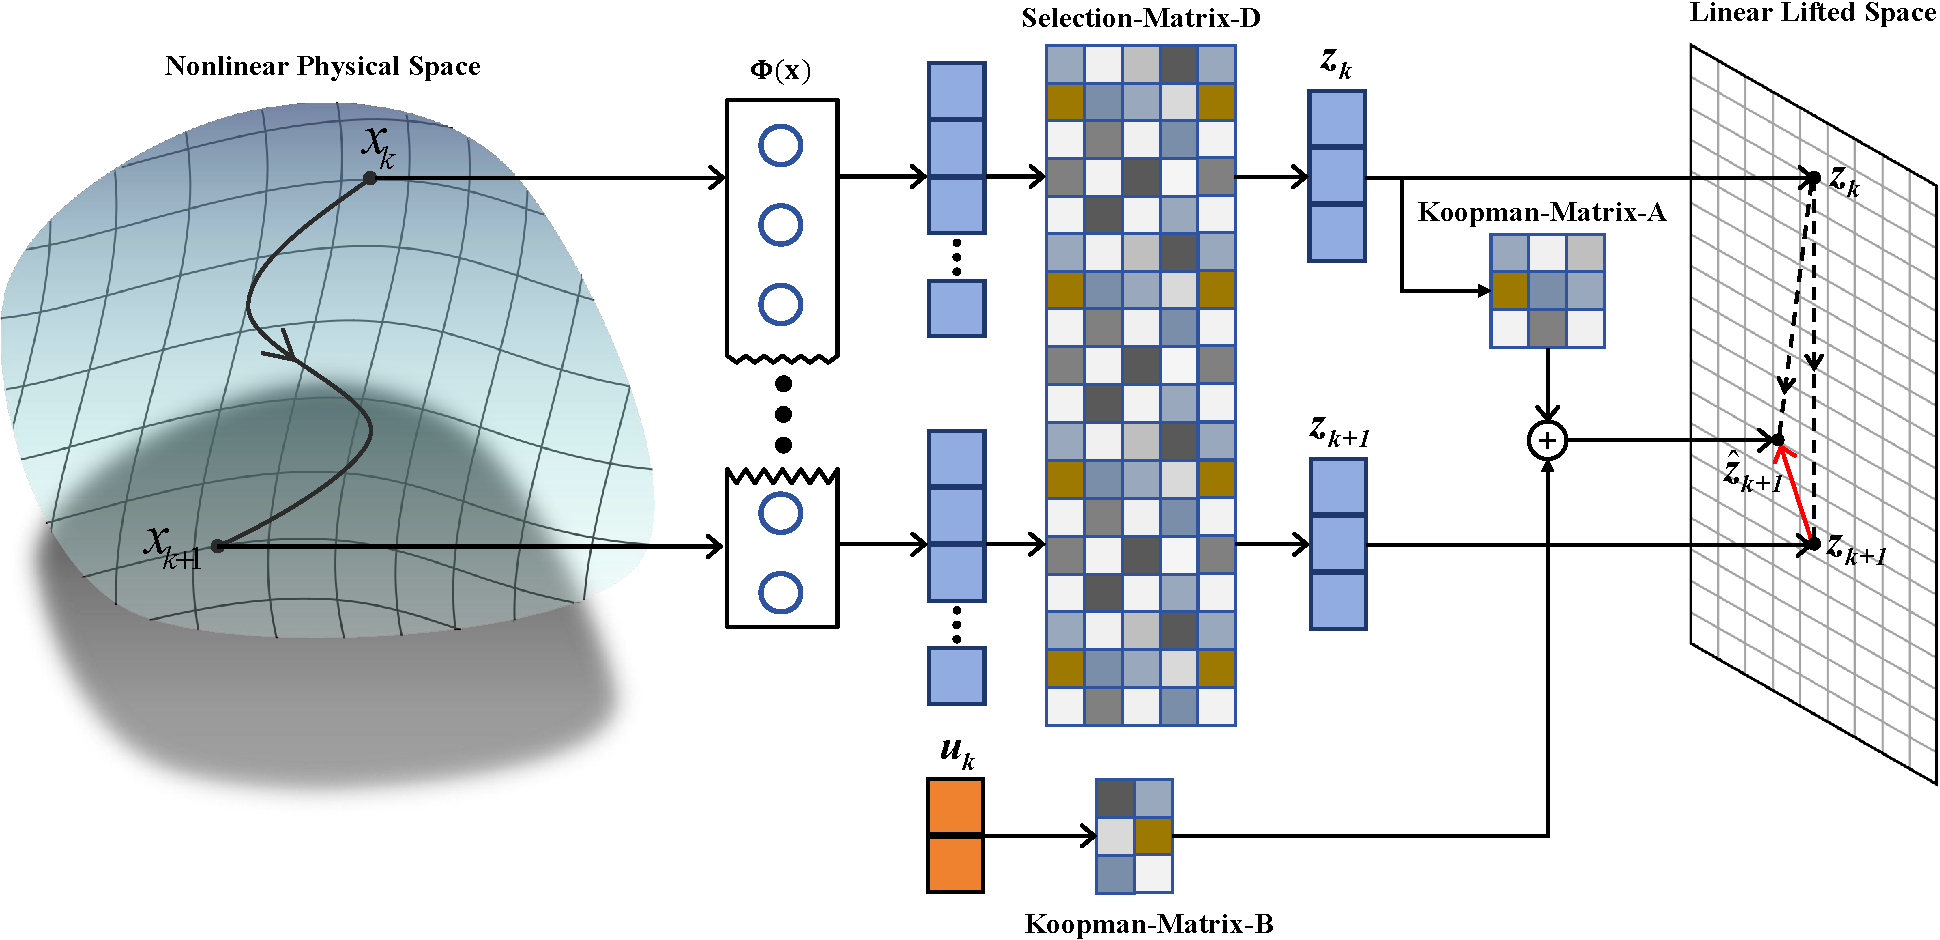
\includegraphics[width=0.85\textwidth]{pictures/Figure1.pdf}
\caption{Koopman representation learning with the learnable feature selection mechanism.}
\label{fig:koopman_framework}
\end{figure*}

Given a trajectory dataset $\{\x_k, \uvec_k\}_{k=1}^{T+1}$, where $\x_k \in \R^n$ represents the robot state (e.g., joint positions and velocities) and $\uvec_k \in \R^m$ denotes the control torque applied to each joint, which yields $T$ one-step transition pairs, we construct the state snapshot matrices $\X = [\x_1, \dots, \x_T]$ and $\Y = [\x_2, \dots, \x_{T+1}]$, the input matrix $\Umat = [\uvec_1, \dots, \uvec_T]$, and the feature matrices $\XPhi = [\Phib(\x_1), \dots, \Phib(\x_T)]$ and $\YPhi = [\Phib(\x_2), \dots, \Phib(\x_{T+1})]$. For a given $\Dmat$, the lifted state data matrices are defined as
\begin{equation}
\Zmat(\Dmat) =
\begin{bmatrix}
\X \\ \Dmat \XPhi
\end{bmatrix}, \qquad
\Zmat^+(\Dmat) =
\begin{bmatrix}
\Y \\ \Dmat \YPhi
\end{bmatrix}.
\end{equation}
We formulate the joint optimization problem as
\begin{equation}
\label{eq:objective}
\begin{aligned}
L(\Kmat,\Dmat) &= \frac{1}{2}
\left\|
\Zmat^+(\Dmat) - \Kmat
\begin{bmatrix}
\Zmat(\Dmat) \\ \Umat
\end{bmatrix}
\right\|_F^2 \\
&\quad + \lambda\|\Dmat\|_1 + \beta\|\Kmat\|_F^2, \\
(\Kmat^\star, \Dmat^\star) &= \arg\min_{\Kmat,\Dmat} \; L(\Kmat,\Dmat).
\end{aligned}
\end{equation}
where $\lambda>0$ and $\beta>0$ are the regularization coefficients. The $\ell_1$ regularization on $\Dmat$ promotes sparse linear combinations of informative candidate functions from the overcomplete candidate function library. Meanwhile, the objective function enforces accurate one-step prediction of both the physical state and the projected feature components in the lifted state, thereby discouraging trivial solutions for $\Dmat$. When $\Dmat = \I_P$ and the regularization terms $\lambda\|\Dmat\|_1$ and $\beta\|\Kmat\|_F^2$ are removed, the formulation reduces to standard EDMD.

Since the optimization problem in~\eqref{eq:objective} is nonconvex in
the joint variables $(\Kmat,\Dmat)$, we adopt a two-block coordinate
descent (BCD) algorithm~\cite{Tseng2001} to solve it by alternately
updating the two variable blocks. Let $(\Kmat^{(t)},\Dmat^{(t)})$
denote the iterates at iteration $t$, and define the corresponding objective value as
\[
L^{(t)} := L(\Kmat^{(t)},\Dmat^{(t)}).
\]
At each iteration, the two variable blocks are updated alternately by solving a strongly convex $\Kmat$-subproblem and a convex $\Dmat$-subproblem.

\textit{1) $\Kmat$-subproblem:}
With $\Dmat^{(t)}$ fixed, define
\[
\mathbf{Y}_{\mathrm{aug}}^{(t)} := \Zmat^+(\Dmat^{(t)}), \qquad
\W^{(t)} :=
\begin{bmatrix}
\Zmat(\Dmat^{(t)}) \\ \Umat
\end{bmatrix}.
\]
Then, the $\Kmat$-subproblem is given by
\[
\min_{\Kmat} \;
\frac{1}{2}\|\mathbf{Y}_{\mathrm{aug}}^{(t)}
- \Kmat \W^{(t)}\|_F^2
+ \beta\|\Kmat\|_F^2 .
\]
This is a standard ridge regression problem. Setting the gradient with respect to $\Kmat$ to zero gives
\[
-(\mathbf{Y}_{\mathrm{aug}}^{(t)} - \Kmat \W^{(t)})
\W^{(t)\top} + 2\beta\Kmat = \mathbf{0},
\]
from which the closed-form update is derived as
\begin{equation}
\label{eq:K_update}
\Kmat^{(t+1)}
= \Zmat^+(\Dmat^{(t)}) \W^{(t)\top}
\bigl( \W^{(t)} \W^{(t)\top} + 2\beta \I \bigr)^{-1}.
\end{equation}

For the $\Kmat$ update, the ridge regularization makes the subproblem strongly convex for any fixed $\Dmat^{(t)}$ and $\beta>0$, so the minimizer in~\eqref{eq:K_update} is unique.

\textit{2) $\Dmat$-subproblem:} With $\Kmat^{(t+1)}$ fixed, the $\Dmat$-subproblem is formulated as
\begin{equation}
\label{eq:D_subproblem}
\Dmat^{(t+1)} = \arg\min_{\Dmat} \; J^{(t)}(\Dmat),
\end{equation}
where
\begin{equation}
\label{eq:D_objective}
J^{(t)}(\Dmat) = \frac{1}{2}\left\| \Zmat^+(\Dmat) - \Kmat^{(t+1)}
\begin{bmatrix}
\Zmat(\Dmat) \\ \Umat
\end{bmatrix} \right\|_F^2
+ \lambda\|\Dmat\|_1.
\end{equation}
To see this, we write $\Kmat^{(t+1)} = [\A^{(t+1)},\B^{(t+1)}]$ and partition $\A^{(t+1)}$ according to the augmented state structure. Since both $\Zmat(\Dmat)$ and $\Zmat^+(\Dmat)$ depend affinely on $\Dmat$, the residual
\[
\Zmat^+(\Dmat) - \Kmat^{(t+1)}
\begin{bmatrix}
\Zmat(\Dmat) \\ \Umat
\end{bmatrix}
\]
is affine in $\Dmat$. Hence, the data-fitting term in~\eqref{eq:D_objective} is a convex quadratic function of $\Dmat$, and the subproblem can be efficiently solved using proximal gradient methods~\cite{Beck2009ISTA}.

For the $\Dmat$ update, the subproblem in~\eqref{eq:D_subproblem} is a convex composite optimization problem consisting of a quadratic data-fitting term and a separable $\ell_1$ regularizer. Hence, it can be solved by standard proximal gradient updates.

Let $T_{\max}$ denote the maximum number of iterations and let $\varepsilon>0$ denote the convergence tolerance. The above block structure leads to the BCD procedure summarized in Algorithm~\ref{alg:altmin}. Its convergence property is stated as follows.

\begin{theorem}[Convergence of the BCD Algorithm]
\label{thm:altmin_convergence}
Suppose that $\lambda>0$ and $\beta>0$, and that each subproblem is solved to optimality at every iteration. Then the sequence $\{(\Kmat^{(t)}, \Dmat^{(t)})\}$ generated by Algorithm~\ref{alg:altmin} satisfies:
\begin{enumerate}
\item The objective values $L^{(t)}$ are monotonically nonincreasing and converge to a finite limit;
\item The iterates $\{(\Kmat^{(t)},\Dmat^{(t)})\}$ remain bounded;
\item Every accumulation point of the sequence is a first-order stationary point of~\eqref{eq:objective}.
\end{enumerate}
\end{theorem}

\begin{proof}
First, since each block is minimized exactly while the other block is fixed, the two successive updates in Algorithm~\ref{alg:altmin} yield
\[
\begin{aligned}
L(\Kmat^{(t+1)},\Dmat^{(t)}) &\le L(\Kmat^{(t)},\Dmat^{(t)}), \\
L(\Kmat^{(t+1)},\Dmat^{(t+1)}) &\le L(\Kmat^{(t+1)},\Dmat^{(t)}).
\end{aligned}
\]
Therefore, $L^{(t+1)} \le L^{(t)}$, and the objective sequence is monotonically nonincreasing. Since $L(\Kmat,\Dmat) \ge 0$, it converges to a finite limit.

Second, from $L^{(t)} \le L^{(0)}$ and the nonnegativity of the data-fitting term, we obtain
\[
\beta\|\Kmat^{(t)}\|_F^2 + \lambda\|\Dmat^{(t)}\|_1 \le L^{(0)}.
\]
Hence, both sequences $\{\Kmat^{(t)}\}$ and $\{\Dmat^{(t)}\}$ are bounded, because boundedness in the $\ell_1$ norm implies boundedness in the Frobenius norm for finite-dimensional matrices.

Finally, the objective in~\eqref{eq:objective} is the sum of a continuously differentiable data-fitting term and a convex separable nonsmooth regularization term, and each block subproblem is solved to optimality at every iteration. By the standard convergence results for block coordinate descent applied to nonsmooth objectives~\cite{Tseng2001}, every accumulation point of $\{(\Kmat^{(t)},\Dmat^{(t)})\}$ is a first-order stationary point of~\eqref{eq:objective}.
\end{proof}

\begin{algorithm}[htbp]
\caption{Feature-Selection BCD Algorithm}
\label{alg:altmin}
\begin{algorithmic}[1]
\REQUIRE Data $(\X,\Y,\Umat)$, basis library $\Phib$, parameters $\lambda,\beta$, initialization $\Dmat^{(0)}$
\ENSURE Learned $\Kmat^\star$ and $\Dmat^\star$
\FOR{$t = 0, 1, \dots, T_{\max}-1$}
    \STATE Update $\Kmat^{(t+1)}$ using~\eqref{eq:K_update}
    \STATE Update $\Dmat^{(t+1)}$ by solving~\eqref{eq:D_subproblem} via a proximal gradient method
    \IF{$|L^{(t+1)} - L^{(t)}| < \varepsilon$}
        \STATE \textbf{break}
    \ENDIF
\ENDFOR
\end{algorithmic}
\end{algorithm}

% ---------------------------------------------------------
\subsection{Lumped Disturbance Analysis}
\label{subsec:error_quantification}
% ---------------------------------------------------------

The learned Koopman model captures the dominant system dynamics, but the finite-dimensional lifted model inevitably contains approximation residuals. In addition, sensor noise and environmental disturbances may appear during robot operation. We collect these effects into a lumped disturbance term $\w_k$, and the actual evolution in the lifted space is written as
\begin{equation}
\label{eq:lumped_model}
\z_{k+1} = \A\z_k + \B\uvec_k + \w_k,
\end{equation}
where $\A$ and $\B$ are the learned Koopman state-transition matrix and input matrix, respectively, obtained from Algorithm~\ref{alg:altmin}.

For compact state-input sets, the Koopman approximation error is theoretically bounded~\cite{Korda2018MPC}. Sensor noise and environmental disturbances are bounded in practical robotic systems due to hardware limits and operating conditions. This motivates the following assumption.

{
\begin{assumption}[Bounded lumped disturbance]
\label{assump:bounded_disturbance}
There exists a constant $\delta_w>0$ such that the lumped disturbance in~\eqref{eq:lumped_model} satisfies
\begin{equation}
\|\w_k\| \le \delta_w, \quad \forall k.
\end{equation}
\end{assumption}
}

Assumption~\ref{assump:bounded_disturbance} links the learned Koopman model to the robust tracking analysis. A smaller approximation residual corresponds to a smaller admissible disturbance level, which is reflected in the ultimate tracking bound derived in Section~\ref{subsec:lqr_robust}.


% =========================================================
\section{LQR Control Based on Koopman Model}
\label{sec:lqr}
% =========================================================

This section designs a feedforward-feedback Koopman-LQR controller for the disturbed lifted model~\eqref{eq:lumped_model} and establishes the ultimate boundedness of the closed-loop tracking error.

\begin{figurehere}
\centering
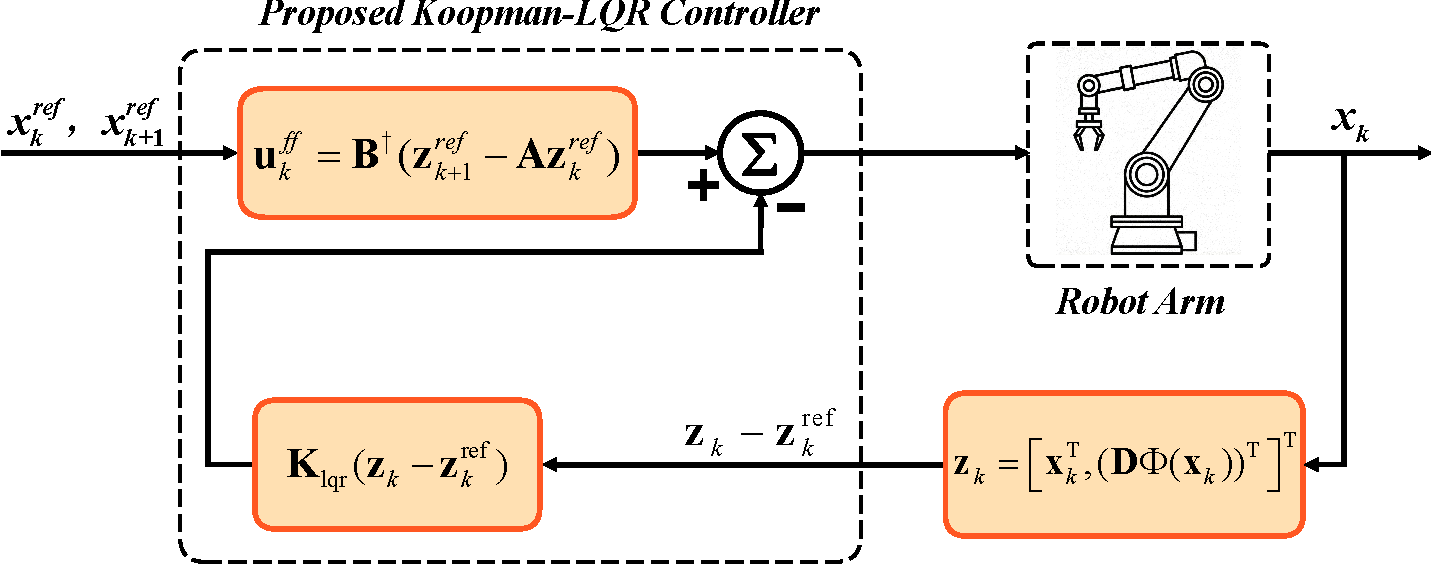
\includegraphics[width=\columnwidth]{pictures/Figure2.pdf}
\caption{\raggedright Structure of the proposed Koopman-based feedforward-feedback LQR controller.}
\label{fig:controller}
\end{figurehere}

\subsection{Feedforward-Feedback Robust Controller Design}
\label{subsec:lqr_design}

To achieve robust trajectory tracking, we design the controller based on the disturbed augmented linear model~\eqref{eq:lumped_model} obtained from the learned Koopman model in Section~\ref{sec:koopman}.
First, let $\{\x_k^{\text{ref}}\}_{k=0}^{\infty}$ denote the desired reference trajectory in the physical state space. By lifting this trajectory through the feature mapping and the learned selection matrix $\Dmat^\star$, we obtain the corresponding lifted reference trajectory:
\begin{equation}
\z_k^{\text{ref}} = [{\x_k^{\text{ref}}}^\top, {(\Dmat^\star\Phib(\x_k^{\text{ref}}))}^\top]^\top.
\end{equation}

To balance the tracking accuracy and the control efforts, we define the following infinite-horizon quadratic cost function:
\begin{equation}
\label{eq:lqr_cost}
J = \sum_{k=0}^{\infty} \left( (\z_k - \z_k^{\text{ref}})^\top \Q (\z_k - \z_k^{\text{ref}}) + \uvec_k^\top \Rmat \uvec_k \right),
\end{equation}
where $\Q = \C^\top \Q_x \C \succeq 0$ is the lifted-state weight matrix, $\Q_x$ is the weight matrix in the original state space, and $\Rmat \succ 0$ is the control input weight matrix.


Assume that the physical system is controllable and that the training data are sufficiently informative such that the learned linear model $(\A,\B)$ is stabilizable. Under these conditions, the standard LQR theory yields a unique optimal state-feedback gain $\Kmat_{\text{lqr}}$, which renders the closed-loop matrix $\A_{\text{cl}} = \A - \B\Kmat_{\text{lqr}}$ Schur stable.

To guarantee the trajectory tracking of the robots, we propose the following composite feedforward-feedback control law:
\begin{equation}
\label{eq:lqr_total}
\uvec_k = \uvec_k^{\mathrm{ff}} - \Kmat_{\text{lqr}}(\z_k - \z_k^{\text{ref}}).
\end{equation}
The feedforward term $\uvec_k^{\mathrm{ff}}$ is used to compensate for the known dynamics along the reference trajectory and is computed as
\begin{equation}
\label{eq:uff}
\uvec_k^{\mathrm{ff}} = \B^{\dagger}(\z_{k+1}^{\text{ref}} - \A\z_k^{\text{ref}}),
\end{equation}
where $\B^{\dagger}$ denotes the Moore-Penrose pseudoinverse of $\B$. Figure~\ref{fig:controller} illustrates the structure of the proposed Koopman-LQR controller.

\subsection{Stability Analysis}
\label{subsec:lqr_robust}

Based on the feedforward-feedback controller~\eqref{eq:lqr_total}, we present the following stability result.

The key observation is that the feedforward term removes the nominal reference dynamics, whereas the LQR feedback stabilizes the deviation around the lifted reference trajectory. Therefore, the closed-loop tracking error can be analyzed as a stable linear system driven by the lumped disturbance.

\begin{theorem}[Robust Tracking Performance]
\label{thm:lqr_uub}
Consider the system~\eqref{eq:lumped_model} under the control law~\eqref{eq:lqr_total}. Suppose that Assumption~\ref{assump:bounded_disturbance} holds. Then the closed-loop system achieves ultimately uniformly bounded (UUB) tracking, i.e., there exists $R > 0$ such that, for any initial condition, there exists a finite time $K$ for which $\|\e_k\| \le R$ for all $k \ge K$.
\end{theorem}

\begin{proof}
Define the tracking error as $\e_k := \z_k - \z_k^{\text{ref}}$. Substituting the control law~\eqref{eq:lqr_total} into the disturbed augmented model~\eqref{eq:lumped_model}, and using the definition of the feedforward term in~\eqref{eq:uff}, the closed-loop error dynamics are given by
\begin{equation}
\label{eq:error_dynamics}
\e_{k+1} = (\A - \B\Kmat_{\text{lqr}})\e_k + \w_k = \A_{\text{cl}}\e_k + \w_k,
\end{equation}
where $\A_{\text{cl}} := \A - \B\Kmat_{\text{lqr}}$ denotes the closed-loop system matrix. By the stabilizability assumption in Section~\ref{subsec:lqr_design} and the standard LQR theory, $\A_{\text{cl}}$ is Schur stable. Hence, there exist positive definite matrices $\mathbf{P} \succ 0$ and $\mathbf{S} \succ 0$ satisfying the discrete-time Lyapunov equation
\[
\A_{\text{cl}}^\top \mathbf{P} \A_{\text{cl}} - \mathbf{P} = -\mathbf{S}.
\]
Consider the Lyapunov function $V_k = \e_k^\top \mathbf{P} \e_k$. Then, along the trajectories of~\eqref{eq:error_dynamics},
\begin{align}
\Delta V_k &= V_{k+1} - V_k \nonumber \\
&= \e_k^\top (\A_{\text{cl}}^\top \mathbf{P} \A_{\text{cl}} - \mathbf{P}) \e_k
+ 2\e_k^\top \A_{\text{cl}}^\top \mathbf{P}\w_k
+ \w_k^\top \mathbf{P}\w_k \nonumber \\
&= -\e_k^\top \mathbf{S} \e_k
+ 2\e_k^\top \A_{\text{cl}}^\top \mathbf{P}\w_k
+ \w_k^\top \mathbf{P}\w_k,
\end{align}
where the last equality follows from the discrete-time Lyapunov equation. By the boundedness of $\w_k$ and the Cauchy--Schwarz inequality, it follows that when $\|\e_k\|$ exceeds a threshold $R$ determined by $\delta_w$, one has $\Delta V_k < 0$. Therefore, the error trajectory enters and remains within the bounded set $\mathcal{B}_R = \{\e : \|\e\| \le R\}$~\cite{Blanchini2008,Khalil2002}.
\end{proof}

Since the projection matrix $\C$ satisfies $\|\C\| = 1$, the error bound in the lifted space directly guarantees the tracking accuracy in the original state space:
\[
\|\x_k - \x_k^{\text{ref}}\| = \|\C\e_k\| \le \|\e_k\| \le R.
\]
Furthermore, the steady-state error bound can be upper bounded by a linear function of the disturbance level, i.e.,
\[
R \le c\,\delta_w,
\]
where the constant $c > 0$ depends only on the spectral properties of the closed-loop matrix $\A_{\text{cl}}$~\cite{Blanchini2008}. This relationship connects the Koopman modeling accuracy with the closed-loop performance: reducing the approximation component of $\w_k$ decreases $\delta_w$ and hence shrinks the ultimate tracking bound.



% =========================================================
\section{Experimental Validations}
\label{sec:experiments}
% =========================================================


% ---------------------------------------------------------
\subsection{Experimental Platforms and Data Collection}
\label{subsec:exp_setup}
% ---------------------------------------------------------

The experiments were conducted on the two platforms shown in Fig.~\ref{fig:experimental_platforms}: a rigid Geomagic Touch\textsuperscript{\textregistered} robot arm and a planar cable-driven soft robotic platform. The robotic arm consists of three revolute joints equipped with integrated encoders for measuring joint positions and velocities. Its force-feedback stylus was fixed during experiments to isolate the joint-space dynamics. The soft robotic platform is composed of a flexible tube actuated by four independently controlled cables driven by stepper motors. A red laser source mounted on the tube projects a light spot onto a projection plate, while a fixed RGB camera captures the spot motion. The corresponding drive electronics, including the controller board and power supplies, are shown in the lower-left panel of Fig.~\ref{fig:experimental_platforms}. For the soft platform, the laser spot position was extracted through HSV-based image segmentation and image-moment localization, and a homography calibrated using four colored markers was used to transform image coordinates into physical $xy$ coordinates.

\begin{figurehere}
\centering
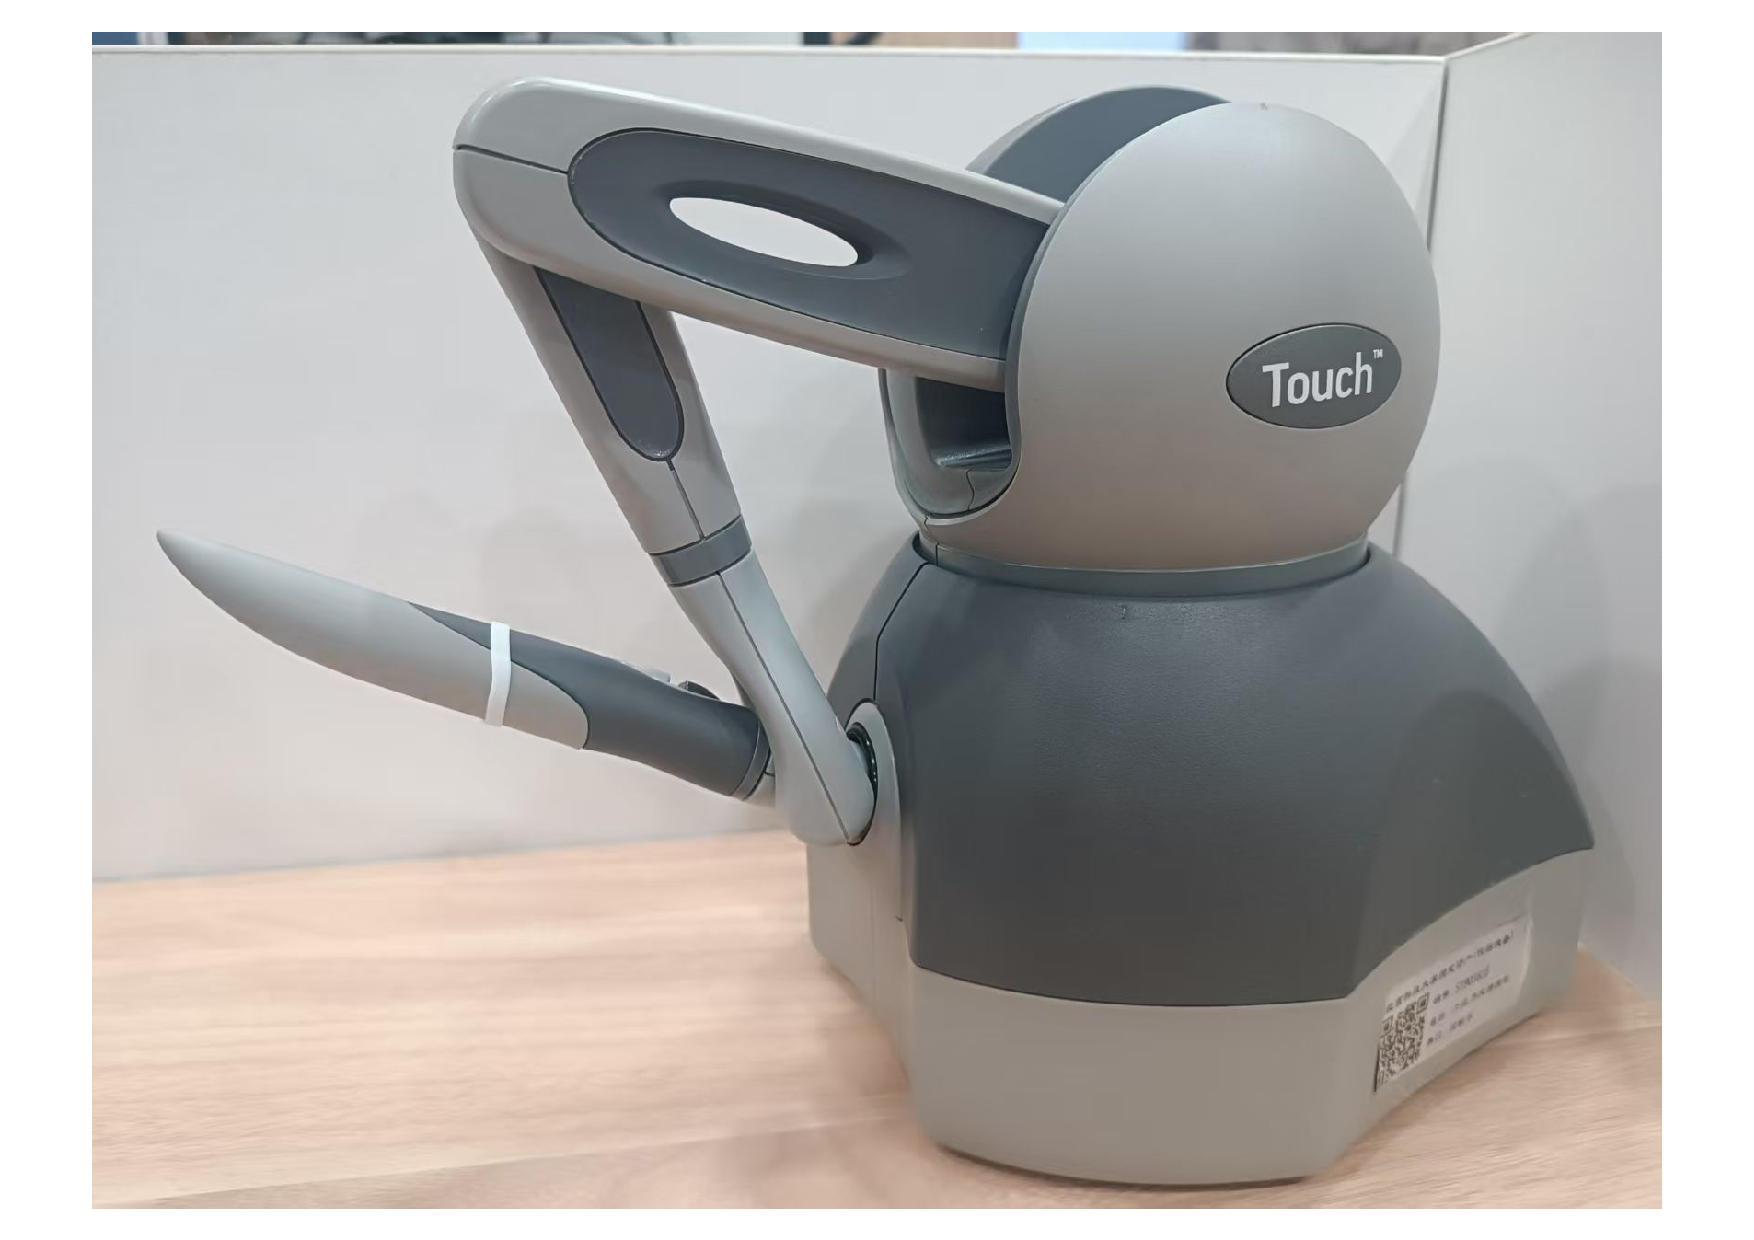
\includegraphics[width=1.0\columnwidth]{pictures/Figure3.pdf}
\caption{\raggedright Experimental setup: the Geomagic Touch robot arm and its drive electronics (left), and the planar cable-driven soft robotic platform (right).}
\label{fig:experimental_platforms}
\end{figurehere}

For both platforms, randomly generated control inputs were applied to excite the system dynamics and collect state trajectories. For the robotic arm, continuous random control torques were applied with a sampling period of 0.004~s, resulting in 20 trajectories of 20~s each containing joint positions, velocities, and control inputs. For the soft robotic platform, random two-dimensional cable-motion commands were applied with a sampling period of 0.2~s, producing 100 trajectories of 60~s each consisting of the two-dimensional light-spot positions and corresponding cable-motion commands. The collected datasets were split at the trajectory level into training, validation, and test sets. Specifically, the robotic-arm dataset was divided using a 15:4:1 ratio, while the soft-platform dataset followed a fixed 70/20/10 split.


% ---------------------------------------------------------
\subsection{Model Prediction Accuracy Comparison}
\label{subsec:modeling_accuracy}
% ---------------------------------------------------------

For comparison, two Koopman-based baselines were considered: EDMDDL~\cite{Li2017}, which learns a low-dimensional dictionary through a feedforward neural network, and standard EDMD~\cite{Williams2015EDMD}, which directly uses the complete candidate function library. FS-EDMD employs the same candidate library as EDMD while learning a compact selection matrix to construct the reduced Koopman representation. All methods were trained and evaluated using the same trajectory-level data splits described in Section~\ref{subsec:exp_setup}.

\begin{figurehere}
\centering
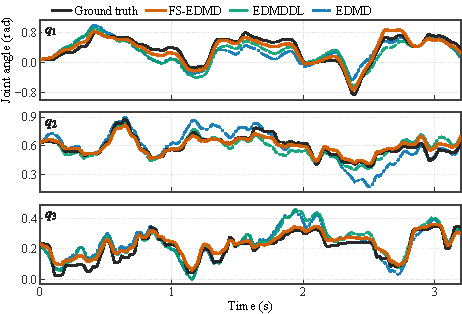
\includegraphics[width=\columnwidth]{pictures/Figure4.pdf}
\caption{Prediction results of the robotic arm over an 800-step rollout. The predicted joint trajectories are compared with the measured trajectories for Joint 1--3.}
\label{fig:robotic_modeling}
\end{figurehere}

\begin{figurehere}
\centering
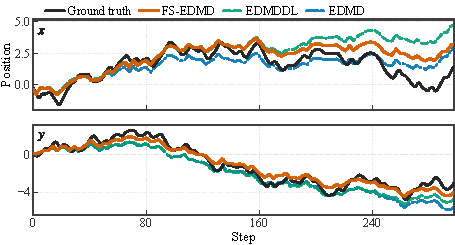
\includegraphics[width=\columnwidth]{pictures/Figure5.pdf}
\caption{Prediction results of the cable-driven soft robotic platform on test trajectory 66. The predicted and measured light-spot positions are compared in the $x$ and $y$ directions.}
\label{fig:soft_modeling}
\end{figurehere}

The lifting dimensions were selected independently for the two platforms. For the robotic arm, the candidate library contains 364 basis functions, and both EDMDDL and FS-EDMD use a 60-dimensional Koopman representation. For the soft robotic platform, the candidate library contains 112 basis functions, and both methods use a 40-dimensional Koopman representation. Therefore, the comparison with EDMDDL evaluates the effectiveness of feature selection under the same reduced dimension, while the comparison with EDMD evaluates the benefit of reducing the lifting space.

The prediction results on both robotic platforms are shown in Fig.~\ref{fig:robotic_modeling} and Fig.~\ref{fig:soft_modeling}. Despite the different dynamic characteristics of the two systems, FS-EDMD consistently provides closer agreement with the measured trajectories over the prediction horizon. Compared with EDMD and EDMDDL, FS-EDMD exhibits reduced prediction deviation for both joint-space motion of the robotic arm and Cartesian light-spot motion of the soft platform, demonstrating the effectiveness of the learned feature selection in constructing compact Koopman representations.

\begin{tablehere}
\centering
\caption{State prediction accuracy comparison of different Koopman models.}
\label{tab:modeling_accuracy}
\small
\setlength{\tabcolsep}{3pt}
\begin{tabular}{llccc}
\toprule
Platform & Method & MSE & RMSE & MAE \\
\midrule
\multirow{3}{*}{Robotic arm}
    & FS-EDMD & \textbf{0.3520} & \textbf{0.5933} & \textbf{0.3202} \\
    & EDMDDL & 0.5936 & 0.7704 & 0.4550 \\
    & EDMD & 0.7256 & 0.8518 & 0.5022 \\
\midrule
\multirow{3}{*}{Soft platform}
    & FS-EDMD & \textbf{0.6224} & \textbf{0.7889} & \textbf{0.5767} \\
    & EDMD & 0.8037 & 0.8965 & 0.7148 \\
    & EDMDDL & 1.6711 & 1.2927 & 0.9368 \\
\bottomrule
\end{tabular}
\end{tablehere}

The quantitative comparison is summarized in Table~\ref{tab:modeling_accuracy}.\footnotemark\ FS-EDMD achieves the lowest prediction errors on both platforms, outperforming both the full-library EDMD model and the neural-network-based dictionary learning approach. These results verify that the proposed feature-selection strategy can identify informative lifting functions and achieve accurate state prediction with a compact Koopman representation.

\footnotetext{\label{fn:pred_metrics}\raggedright
$\mathrm{MSE} = \frac{1}{T}\sum_{k=1}^{T}\|\x_k - \hat{\x}_k\|^2$,
$\mathrm{RMSE} = \sqrt{\mathrm{MSE}}$,
$\mathrm{MAE} = \frac{1}{T}\sum_{k=1}^{T}\|\x_k - \hat{\x}_k\|$,
where $\hat{\x}_k$ denotes the predicted state at time step $k$. Robotic-arm metrics are computed over joint positions and velocities, whereas soft-platform metrics are computed over the two-dimensional light-spot position.
}


% ---------------------------------------------------------
\subsection{Trajectory Tracking Control Performance Evaluation}
\label{subsec:control_performance}
% ---------------------------------------------------------

Trajectory tracking experiments were conducted on both robotic platforms to evaluate the effectiveness of the proposed FS-EDMD-LQR controller in closed-loop control. The controller employed the feedforward-feedback structure described in Section~\ref{sec:lqr}. For the robotic arm, the weighting matrices were set to $\Q=\mathrm{diag}(100,10,100,10,100,10)$ and $\Rmat=\I_3$, while a PID controller with empirically tuned gains of $K_p=25$, $K_i=0.1$, and $K_d=2.5$ was used as the baseline. For the soft robotic platform, FS-EDMD-LQR used $\Q_x=\mathrm{diag}(250,250)$ and $\Rmat=\I_2$, and the PID controller used gains of $K_p=20$, $K_i=1$, and $K_d=10$. All tracking errors were evaluated over the same time intervals after controller initialization to ensure a fair comparison.

\begin{figurehere}
\centering
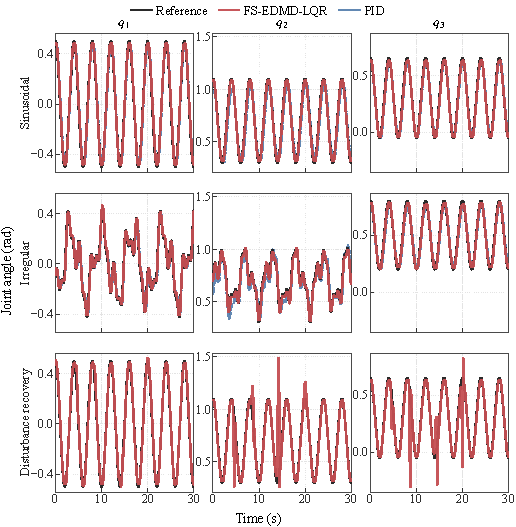
\includegraphics[width=\columnwidth]{pictures/Figure6.pdf}
\caption{Robotic-arm trajectory tracking results under sinusoidal, irregular, and disturbance-recovery references. The first two rows compare FS-EDMD-LQR and PID tracking performance, while the third row shows the disturbance-recovery response of FS-EDMD-LQR.}
\label{fig:control_tracking}
\end{figurehere}

\begin{figurehere}
\centering
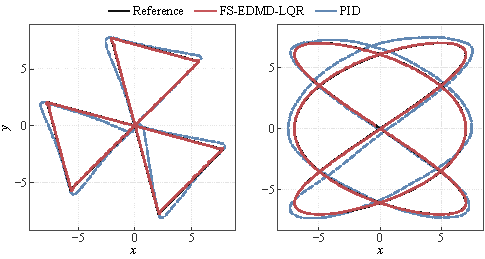
\includegraphics[width=\columnwidth]{pictures/Figure7.pdf}
\caption{Soft-platform trajectory tracking results for triangle and Lissajous references. The desired trajectories are compared with the responses of FS-EDMD-LQR and PID.}
\label{fig:soft_control_tracking}
\end{figurehere}

The trajectory tracking results for both robotic platforms are presented in Fig.~\ref{fig:control_tracking} and Fig.~\ref{fig:soft_control_tracking}. Although the two systems exhibit different dynamic characteristics, FS-EDMD-LQR consistently achieves closer agreement with the desired trajectories than PID. For the robotic arm, the proposed controller maintains accurate tracking for both sinusoidal and irregular references and provides stable recovery after external disturbances. For the cable-driven soft robotic platform, FS-EDMD-LQR achieves accurate tracking of both triangle and Lissajous trajectories, demonstrating its capability to handle nonlinear and coupled system dynamics.

\begin{tablehere}
\centering
\caption{Trajectory tracking performance comparison.}
\label{tab:control_metrics}
\footnotesize
\setlength{\tabcolsep}{3pt}
\begin{tabular}{llcc}
\toprule
Type & Controller & RMSE & MAE \\
\midrule
\multirow{2}{*}{Arm: sinusoidal}
    & FS-EDMD-LQR & \textbf{0.0154} & \textbf{0.0136} \\
    & PID & 0.0475 & 0.0402 \\
\midrule
\multirow{2}{*}{Arm: irregular}
    & FS-EDMD-LQR & \textbf{0.0175} & \textbf{0.0148} \\
    & PID & 0.0413 & 0.0337 \\
\midrule
Arm: disturbance recovery
    & FS-EDMD-LQR & \textbf{0.0958} & \textbf{0.0298} \\
\midrule
\multirow{2}{*}{Soft: triangle}
    & FS-EDMD-LQR & \textbf{0.1749} & \textbf{0.1703} \\
    & PID & 0.6645 & 0.5468 \\
\midrule
\multirow{2}{*}{Soft: Lissajous}
    & FS-EDMD-LQR & \textbf{0.1266} & \textbf{0.1172} \\
    & PID & 1.7883 & 1.6710 \\
\bottomrule
\end{tabular}
\end{tablehere}

The quantitative tracking results are summarized in Table~\ref{tab:control_metrics}.\footnotemark\ FS-EDMD-LQR achieves consistently lower tracking errors than PID across all evaluated trajectories on both platforms. These results demonstrate that the proposed feature-selected Koopman model provides an effective representation for feedback control, enabling accurate trajectory tracking and robust closed-loop performance under different operating conditions.

\footnotetext{\label{fn:track_metrics}\raggedright
For the robotic arm, 
$\mathrm{RMSE}=\sqrt{\frac{1}{3T}\sum_{i=1}^{3}\sum_{k=1}^{T}(q_i(k)-q_i^{\mathrm{ref}}(k))^2}$ and
$\mathrm{MAE}=\frac{1}{3T}\sum_{i=1}^{3}\sum_{k=1}^{T}|q_i(k)-q_i^{\mathrm{ref}}(k)|$.
For the soft platform,
$\mathrm{RMSE}=\sqrt{\frac{1}{T}\sum_{k=1}^{T}\|\mathbf{p}_k-\mathbf{p}_k^{\mathrm{ref}}\|_2^2}$ and
$\mathrm{MAE}=\frac{1}{T}\sum_{k=1}^{T}\|\mathbf{p}_k-\mathbf{p}_k^{\mathrm{ref}}\|_2$.
The robotic-arm errors are computed in joint space (rad), whereas the soft-platform errors are computed from the two-dimensional light-spot position.
}


% =========================================================
\section{Conclusion}
\label{sec:conclusion}
% =========================================================

This paper proposed a learnable feature-selection framework for EDMD that constructs compact Koopman representations from overcomplete physics-informed candidate libraries. By jointly optimizing the selection matrix and lifted dynamics, the proposed method enables Koopman-LQR control with bounded approximation and disturbance uncertainties. Lyapunov analysis establishes ultimate uniform boundedness of the closed-loop tracking error. Experiments on a three-degree-of-freedom rigid robot arm and a cable-driven soft robotic platform demonstrate improved prediction accuracy and tracking performance compared with EDMD, EDMDDL, and PID baselines, together with robust disturbance recovery. The current study is limited to the tested operating ranges and bounded-disturbance setting. Future work will investigate online adaptation and model predictive control to handle varying dynamics and explicit state/input constraints.




% ================== References ==================
